\documentclass[a4paper,12pt]{article}
\usepackage{amsmath}
\usepackage{multicol}
\usepackage{color}
\usepackage{lipsum}
\usepackage{algorithm}
\usepackage{algpseudocode}
\usepackage[utf8]{inputenc}
\usepackage{hyperref}
\hypersetup{
    colorlinks=true,
    linkcolor=black,
    urlcolor=blue
}
\urlstyle{same}

\usepackage{xecyr}
\usepackage[russian]{babel}
\usepackage[top=20mm, bottom=20mm, left=25mm, right=15mm]{geometry}


%% Графики 
\usepackage{pgfplots}
\usepackage{pgfplotstable}
\usepackage{booktabs}
\usepackage{array}
\usepackage{colortbl}

%% Картинки
\usepackage{graphicx}
\graphicspath{ {./images/} }

\pgfplotstableset{% global config, for example in the preamble
  every head row/.style={before row=\toprule,after row=\midrule},
  every last row/.style={after row=\bottomrule},
  fixed,precision=2
 }

%% Шрифты
\setmainfont{Times New Roman} %CMU Serif}

\definecolor{graylight}{rgb}{0.6, 0.6, 0.6}

%% Свои команды
\DeclareMathOperator{\sgn}{\mathop{sgn}}
\newcommand{\DL}{\newline\newline}

%%% Заголовок
\author{Шамрин Игорь СКБ172}
\title{ Криптосистема с открытым ключом типа рюкзака, основанная на арифметике в конечных полях \DL
\large Перевод статьи BENNY CHOR  и RONALD L. RIVEST}
\date{\today}

\begin{document} 
\thispagestyle{empty}

\begin{center}

\sc
ФЕДЕРАЛЬНОЕ  ГОСУДАРСТВЕННОЕ АВТОНОМНОЕ
ОБРАЗОВАТЕЛЬНОЕ УЧРЕЖДЕНИЕ ВЫСШЕГО ОБРАЗОВАНИЯ
«НАЦИОНАЛЬНЫЙ ИССЛЕДОВАТЕЛЬСКИЙ УНИВЕРСИТЕТ
«ВЫСШАЯ ШКОЛА ЭКОНОМИКИ»
\end{center}

\begin{center}
\bf Московский институт электроники и математики им.~А.Н.~Тихонова
\end{center}

\vspace{1cm}

\begin{center}
Шамрин Игорь Михайлович
\end{center}

\vspace{1cm}

\begin{center}
\bf Перевод статьти BENNY CHOR  и RONALD L. RIVEST "Криптосистема с открытым ключом типа рюкзака, основанная на арифметике в конечных полях"
\end{center}

\vspace{10mm}

\begin{center}
Курсовая работа \par
по специальности 10.05.01 «Компьютерная безопасность» \par
студента образовательной программы специалитета
\end{center}

\vfill

\begin{multicols}{2}
\begin{flushleft}
~Студент\par\:\par
\begin{tabular}{c}
\underline{\hspace{8em}} \vspace{-2mm}\\
{\tiny {\color{graylight}подпись}}
\end{tabular}
\begin{tabular}{c}
\underline{\hspace{2em}Шамрин И.М.\hspace{1em}}\\
{\tiny{\color{graylight} ФИО}}
\end{tabular}
\end{flushleft}

\begin{flushright}
Преподаватель

доцент
\end{flushright}

\begin{tabular}{c}
\underline{\hspace{8em}} \vspace{-1mm}\\
{\tiny {\color{graylight}подпись}}
\end{tabular}
\begin{tabular}{c}
\underline{\hspace{2em}Нестеренко А.Ю.\hspace{1em}} \vspace{-1mm}\\
{\tiny{\color{graylight} ФИО}}
\end{tabular}
\end{multicols}

\vfill
\begin{center}Москва, 2021 г.\end{center}

\newpage

\tableofcontents

\newpage
\begin{abstract}
Представлена новая криптосистема с открытым ключом типа рюкзака. Система основана на новом применении арифметики в конечных полях, следуя конструкции Боза и Чоулы. Правильно выбрав параметры, можно контролировать плотность полученного рюкзака, которая представляет собой соотношение между количеством элементов в рюкзаке и их количеством в битах. В частности, плотность может быть достаточно высокой, чтобы предотвратить атаки “низкой плотности” на нашу систему. На данный момент неизвестно ни одной атаки, способной “взломать” эту систему за разумное время. 
\end{abstract}


\newpage

\section{Введение}

В 1976 году Диффи и Хеллман \cite{11} представили идею криптографии с открытым ключом, в которой используются два разных ключа: один для шифрования и один для дешифрования. Каждый пользователь хранит свой ключ дешифрования в секрете, делая ключ шифрования открытым, поэтому его могут использовать все желающие отправлять ему сообщения. Несколько месяцев спустя,
были обнаружены первые две реализации криптосистем с открытым ключом: схема Меркла-Хеллмана \cite{21} и схема Ривеста-Шамира-Адельмана (RSA) \cite{26}. С тех пор было предложено больше криптосистем с открытым ключом. Большинство из этих реализаций можно разделить на две категории:
\begin{itemize}
  \item[a)] Схемы основанные на сложных теоретико-числовых задачах (например, RSA \cite{26}, Рабин \cite{24}, Уильямс [31], Голд-вассер-Микали \cite{13});
  \item[б)] Схемы, связанные с проблемой рюкзака (например, Меркл-Хеллман \cite{21}, Шамир \cite{30}).
\end{itemize}

\noindent Хотя неизвестно эффективных атак на системы с открытым ключом с теорией чисел, было показано, что несколько систем типа рюкзака небезопасны. Большинство из этих систем имеют скрытую сверхвозрастающую последовательность. Шамир совершил первую успешную атаку на базовую систему Меркла-Хеллмана \cite{29}. После его атаки были предложены другие атаки на более сложные системы. В частности, Брикелл \cite{5} нашел способ нарушить общую схему Меркла-Хеллмана. 

Другой атакой является атака “низкой плотности’ Лагариаса и Одлизко \cite{17}. Плотность рюкзака определяется как отношение количества элементов в нем к размеру (в битах) этих элементов. Наиболее интересным моментом в атаке Лагариаса-Одлизко является то, что она не делает никаких предположений о том, как была построена система, и, следовательно, может быть применима к любой криптосистеме ранцевого типа, плотность которой невелика (в отличие от атаки Шамира, которая в значительной степени опирается на сверхвозрастающую базовую последовательность). Другая атака с низкой плотностью была предложена Брикеллом \cite{4}, хотя на практике она представляется менее эффективной. В результате этих атак криптосистемы рюкзачного типа, которые либо основаны на сверхвозрастающих последовательностях, либо имеют очень низкую плотность, кажутся уязвимыми. 

Хочется отметить, что все известные теоретико-числовые методы криптосистем с открытым ключом не более сложны, чем задача факторизации, и, следовательно, все они сводятся к проблеме взятия дискретных логарифмов в составных модулях (см. \cite{2}, \cite{7}, \cite{19}). Если эта проблема дискретного логарифма станет разрешимой (что сделает все “теоретико-числовые” систем с открытм ключом небезопасными), нашу систему будет проще создавать для рюкзаков еще большего размера.

Остальная часть этой статьи организована следующим образом: В разделе II мы обсуждаем проблему рюкзака и его использование в криптосистемах. Раздел 3 представляет собой описание теоремы Бозе-Чоула и ее доказательства. В разделе IV мы приводим подробную информацию о нашей новой криптосистеме. В разделе V рассматривается производительность системы, а в разделе VI описываются фактические параметры для реализации нашей криптосистемы с публичным ключом. Наконец, некоторые возможные атаки на новую систему анализируются в разделе VII. \DL

\section{Криптосистемы рюкзачного типа}
Задача о рюкзаке 0-1 - это NP-полная задача, которую можно сформулировать следующим образом: пусть дано множество $ A = \{a_i |  0 \leq i \leq n-1\}$ неотрицательных целых чисел и неотрицательное целое число S. Существует ли целочисленное решение уравнения $\sum x_i a_i = S$ где все $a_i$ являются 0 или 1? Дополнительный вариант формулировки задачи состоит в том, чтобы убрать ограничение 0-1 на $x_i$, и ограничить его только неотрицательными целыми числами, ограничив их вес некоторым $h$, таким что $\sum x_i \leq h$.

Криптосистемы с открытым ключом типа рюкзака основаны на невозможности найти решение для $S= \sum x_i a_i$, даже если известно, что решение существует. В таких системах каждый пользователь публикует набор $A$ из $a_i$ и связанный $h$. Простое текстовое сообщение, состоящее из целочисленного вектора $M = (x_0, x_1, ..., x_{n-1})$ с весом $\leq h$ шифруется путем установки 
$$ E(M) = \sum x_i a_i $$

Элементы рюкзака $a_i$ выбраны таким образом, чтобы уравнение легко решалось, если известна определенная информация о секретном люке. Точный характер этой информации зависит от конкретной рассматриваемой системы. Общим свойством рюкзачных систем с открытым ключом является то, что шифрование простое - все, что вам нужно сделать, это сложить. \DL

\section{Криптосистемы рюкзачного типа }
В 1936 году Сайдон поднял вопрос о том, существуют ли “плотные” последовательности, h-кратные суммы которых уникальны. Учитывая $n$ и $h$, неотрицательные целые числа, существует ли последовательность $ A = \{a_i |  0 \leq i \leq n-1\}$, состоящая из неотрицательных целых чисел, такая что все суммы, состощяие в точности из $h$ элементов (допускаются повторения) из $A$ различны? Легко построить такие последовательности, если $a_i$, растут экспоненциально в $n$. Например, последовательность $\{1, h, h^2, ..., h^{n-1}\}$ обладает вышеупомянутым свойством (но не работает даже для сумм из $h+1$ элементов, т.к. $h^2 + h*1 = (h+1)*h$)). Однако можно ли построить такие последовательности из $a_i$, растущим только полиномиально быстро в n? Бозе и Чоула \cite{3} нашли очень элегантный способ построения таких последовательностей с $1 \leq\ a_i \leq n^h -1$ для всех $0 \leq i \leq n-1$ См. Халберстама и Рота \cite{14} [гл.21]. Здесь мы представляем слегка измененную версию теоремы Бозе-Чаулы, которая хорошо согласуется с нашим криптографическим приложением.

\textsl{Теорема Бозе-Чоула}: Пусть дано простое число $p$ и целое $h \geq 2$. Тогда существует последовательность $A = \{a_i | 0\leq i \leq p -1\}$, такая что \newline
\begin{itemize}
  \item[1)] $1 \leq a_i \leq p^h -1, \;\;\; i = 0,1,...,p-1$
  \item[2)] Если $(x_0, x_1, ... , x_{p-1})$ и $(y_0, y_1,...,y_{p-1})$ являются двумя
различными векторами с неотрицательными координатами и $\sum_{i=0}^{p-1}x_i, \sum_{i=0}^{p-1}y_i \leq h$, тогда $\sum_{i=0}^{p-1}x_i a_i \neq \sum_{i=0}^{p-1}y_i a_i$
\end{itemize}

\noindent \textsl{Доказательство}: \newline
Построение происходит в конечном поле $GF(p)$ и его расширении $GF(p^h)$ (для удобства элементы $GF(p)$ будут проиндексированы в соответствии с их лексикографическим порядком). Пусть $t \in GF(p^h)$. Пусть $g -$ пораждающий элемент поля $GF(p^h)$ (т.е. $GF(p^h)^* = \{ g^e | - \leq e \leq p^h - 1 \}$). Рассмотрим аддитивный сдвиг на t поля $GF(p)$, а именно на множество 
$$ t + GF(p) = \{t + \alpha_i|\alpha_i \in GF(p) \} \subset GF(p^h). $$ 

Пусть $a_i = \log_g{(t + \alpha_i)} (\alpha_i \in GF(p)$ является логарифмом от $t + \alpha_i$ для $g \in GF(p^h).$ Тогда $a_i$, все целые числа в интервале $[l, p^h - 1]$ и они удовлетворяют различимости $h-$кратных сумм. Предположим, что есть два вектора $\Vec{x}, \Vec{y}$ неотрицательных целых чисел, удовлетворяющих \eqref{eq:1}, \eqref{eq:2} и \eqref{eq:3}:

\begin{equation}
(x_0, x_1, ... , x_{p-1}) \neq (y_0, y_1, ..., y_{p-1}) \label{eq:1} 
\end{equation} 
\begin{equation}
\sum_{i = 0}^{p-1}x_i, \sum_{i = 0}^{p-1}y_i \leq h \label{eq:2} 
\end{equation} 
\begin{equation}
\sum_{i = 0}^{p-1}x_i a_i = \sum_{i = 0}^{p-1}y_i a_i\label{eq:3} 
\end{equation} 

Тогда выполняется следующие равенство в $GF(p^h)$: \newline
$$g^{\sum_{i = 0}^{p-1}x_i y_i} = g^{\sum_{i = 0}^{p-1}y_i y_i}$$
и тогда 
$$ \prod_{i = 0}^{p-1}(g^{a_i^{x_i}}) = \prod_{i = 0}^{p-1}(g^{a_i^{y_i}}) $$

Используя свойство $g^{a_i} = t + \alpha_i$ и полагая только ненулевые $x_i, y_i$, получаем 
$$ (t+\beta_1)^{x_1}(t+\beta_2)^{x_2})...(t+\beta_l)^{x_l} = (t+\gamma_1)^{y_1}(t+\gamma_2)^{y_2})...(t+\gamma_m)^{y_m}$$
где ${\beta_1,\beta_2, ..., \beta_l}$ и ${\gamma_1,\gamma_2, ..., \gamma_m}$ являются двумя разными непустыми подмножествами $GF(p)$ с не более чем $h$ элементами каждый. Таким образом, обе стороны последнего уравнения являются различными моническими многочленами степени $\leq h$ с коэффициентами в $GF(p)$, так, вычитая их, мы получим что $t$ является корнем ненулевого многочлена степени $\leq h-1$ c коэффициентами в $GF(p)$. Это противоречит тому факту, что $t$ является степенью $h$ в поле $GF(p)$\newline

\textsl{Замечания:} 1) Из доказательства ясно, что суммы $l$ $(l \leq h)$ в $A$ различны не только $Z$, но так же по модулю $p^h - 1$. 2) Требование на простоту $p$ может быть заменено на “$p$ является простой степенью” без изменения утверждения и его доказательства.\DL

\section{Как криптосистемы были сконструированы и использовались}
В этом разделе мы опишем, как создается и используется новая криптосистема. Мы начнем с неформального (и немного упрощенного) описания. Далее приводится пошаговый рецепт создания криптосистемы, шифрования сообщений и расшифровки зашифрованных текстов. Наконец, мы опишем, как преобразовать “обычные” неограниченные битовые строки в строки с фиксированным весом. \newline

\textsl{A. Криптосистема}
\DL
Первый шаг - выбрать простое число (или простую степень) $p$ и $h$ так, чтобы $GF(p^h)$  поддавался вычислениям дискретного логарифма. Мы оставляем $p$ и неуказанные параметры в этом разделе и подробнее остановимся на их точном выборе в разделе VI (приблизительные величины будут $p \approx 200, h \approx 25$). Как только $p$ и $h$ выбраны, мы выбираем $t \in GF(p^h)$ степени $h$ над базовым полем и примитивный элемент $g \in GF(p^h)$ (и $t$, и $g$ выбираются случайным образом из множества возможных кандидатов). Следуя Бозе и Чоуле, вычисляются логарифмы (по основанию $g$) элементов $p$ в $GF(p)+t$. Эти p целых чисел затем шифруются с использованием случайно выбранной перестановки. Зашифрованные целые числа публикуются. Вместе с $p$ и $h$ они составляют открытый ключ шифрования, в то время как элементы $t, g$ и перестановка расшифровки составляют секретный ключ дешифрования. Чтобы зашифровать двоичное сообщение длиной $p$ и весом $h$, пользователь добавляет элементы рюкзака с 1 в соответствующее местоположение сообщения и отправляет сумму. Когда законный получатель получает сумму, он сначала поднимает генератор $g$ до нее и выражает результат в виде многочлена степени $h$ в $t$ над $GF(p)$. Корни $h$ этого многочлена находятся путем последовательных подстановок. Применяя обратную к исходной перестановке, восстанавливаются индексы простого текста, имеющего бит 1. \newline
\textsl {1) Генерация системы}: а) Пусть $p$ - степень простого числа, $h\leq p$, целое число, такое, что дискретные логарифмы в $GF(p^h)$ могут быть эффективно вычислены. \newline
\indent b) Возьмем случайное $t \in GH(p^h)$ такое, что оно является степенью $h$ в $GF(p)$. Это будет сделано путем нахождения $f(t)$, случайного неприводимого монического многочлена степени h в $GF(p)[t]$ и представляющий арифметику $GF(p^h)$ через $GF(p)[t]/<f(t)>$. (То есть элементы $GF(p^h)$ являются многочленами степени $\leq h - 1$ с коэффициентами в $GF(p)$, а операции сложения/умножения выполняются по модулю p и $f(t)$).\newline
\indent c) Выбрать случайное $g \in GF(p^h)$, такое тчоg порождающий элемент поля $GF(p^h)$. Это будет сделано путем выбора случайного параметра $r \in GF(p^h)$ до тех пор, пока не будет найден тот, который удовлетворяет $r^{p^h-1}/s \neq 1$ (для всех простых множителей $s$ из $p^h-1$). Обратите внимание, что в нашей системе $p^h -1$ будет иметь только малые простые делители, и поэтому легко проверить, что данный $r$ проходит вышеуказанный тест. Поскольку плотность таких элементов во всех случаях относительно высока (независимо от каких-либо особых свойств $p$ и $h$), описанная выше процедура действительно выполнима. \newline
\indent d) Построение по теореме Бозе-Чоула: Вычислить $a_i= \log_g(t +a_i)$ для всех $a_i \in GF(p)$. \newline
\indent e)  Переставить $a_i$ : пусть $pi: \{ 0, 1, ..., p-1 \} \rightarrow \{ 0, 1, ..., p-1 \}$ будет случайно выбранной перестановкой. Задать $b_i = a_{\pi(i)}$ \newline
\indent f) Добавить немного шума: выбрать случайное $0\leq d \leq p^h$ 2 случайным образом. Установить $c_i = b_i+d$ \newline
\indent g) Публичный ключ: $c_0, c_1, ..., c_{p-1};p,h$ \newline
\indent h) Приватный ключ: Имеем $t,g,\pi^{-1}, d$ \newline
\textsl{Замечание:} Каждый пользователь может использовать одни и те же $p$ и $h$. Вероятность коллизий (у двух пользователей одинаковые ключи) ничтожно мала. \newline
\indent \textsl{Шифрование: } \newline Чтобы зашифровать двоичное сообщение M = $(x_0,...,x_{p-1})$ длины $p$ и веса (количество единиц) с точностью до $h$, добавьте $c_i$, соответствующий бит которого равен 1. Отправьте
$$E(M) = \sum_{i=0}^{p-1}x_i c_i \quad mod(p^h -1)$$

\textsl{3) Расшифрование}: \newline
\indent a) Пусть $r(t)= t^h$ по модулю $f(t)$, многочлен степени $\leq h - 1$ (вычисляется один раз при генерации системы). \newline
\indent b) Дано $s = E(M)$, вычислить $s' = s-hd$ (по модулю $p^h - 1$) \newline
\indent c) Вычислить $q(t) = g^{s'}$ по модулю $f(t)$, формальный многочлен степени $h -1$ от переменной t. \newline
\indent d) Сложить $t^h - r(t)$ с $q(t)$, получить $s(t) = t^h + q(t) - r(t)$, многочлен степени $h$ в $GF(p)[t]$ \newline
\indent e) Теперь имеем: 
$$s(t) = (t+ \alpha_{i_1}) * (t+ \alpha_{i_2}) ... (t+ \alpha_{i_h})$$
назовите коэффициенты $s(t)$ для линейных членов в $GF(p)$. Путем последовательных замен мы находим $h$ корней $a_{i_j}$ (требуется не более $p$ замен). Примените $\pi^{-1} $ для восстановления координат исходного $M$, имеющего бит 1.\DL

\textsl{B. Преобразование Неограниченных Битовых Строк} \newline
До сих пор мы предполагали, что пространство сообщений $M$ содержит двоичные векторы длины $p$ и веса $h$. Однако обычный двоичный текст не имеет такой формы. В этом подразделе описывается простая процедура перевода неограниченного двоичного текста в вышеупомянутую форму. \newline
\indent Учитывая двоичный текст, мы сначала разбиваем его на блоки по $\Big \lfloor \log_2 
\begin{pmatrix}
  p\\ 
  h
\end{pmatrix}
\Big \rfloor$ каждый. Каждый из этих блоков рассматривается как
двоичное представление числа $n$, $0 \leq n \leq \begin{pmatrix}p\\h\end{pmatrix}$. \newline
Чтобы отобразить эти числа в двоичные векторы веса h, мы используем отображение с сохранением порядка, вызванное лексикографическим порядком векторов и естественным порядком целых чисел. Если $n$ больше чем $\begin{pmatrix}p-1\\h-1\end{pmatrix}$, первый бит соответствующего вектора устанавливается равным 1. В противном случае первый бит устанавливается равным 0. Затем мы обновляем $p$ и $h$ и повторяем $p$ раз, пока не будут определены все $p$ битов: \DL
\indent код для преобразования числа n в двоичный вектор $\Vec{y}$:
\begin{algorithmic}[1]
\For{$i\gets1$ \KwTo $p$}
\If{$n \geq \begin{pmatrix}p-i\\h\end{pmatrix}$}
\State{$y_i \gets 1$}
\State{$n \gets n - \begin{pmatrix}p-i\\h-l\end{pmatrix}$}
\State{$h \gets h-1$}
\Else
\State{$y_i \gets 0$}
\EndIf
\EndFor
\State{\Return{$\Vec{y}$}}
\end{algorithmic}

Обратное преобразование, которое является последним шагом в расшифровке, так же просто: \newline
\indent код для преобразования двоичного вектора $\Vec{y}$ в число $n$:\newline
\indent Вход: {$\Vec{y}$, p, h}; Выход: $n$

\begin{algorithmic}[1]
\State{$n \gets 0$}
\For{$i\gets1$ \KwTo $p$}
\If{$y_i = 1$}
\State{$n \gets n + \begin{pmatrix}p-i\\h\end{pmatrix}$}
\State{$h \gets h-1$}
\EndIf
\EndFor
\State{\Return{$n$}}
\end{algorithmic}


Для эффективной реализации биномиальные коэффициенты $p*h/4$ будут предварительно вычислены и постоянно сохранены. \newline
\indent \textsl{Замечание: } Предыдущая схема индексирования хорошо известна
в литературе (см., Например, \cite{10}). \DL

\section{Производительность системы: время, пространство и скорость передачи информации}
В этом разделе мы анализируем три основных параметра криптосистемы: время, необходимое для шифрования и дешифрования сообщения, размер ключей и скорость передачи информации в битах открытого текста на биты зашифрованного текста. Сложность генерации ключей обсуждается в разделе VI. \newline
\indent
Учитывая длину двоичного сообщения $p$ и вес $h$, его шифрование равносильно добавлению $h$ целых чисел $c_i$, каждое из которых меньше $p^h$. Время выполнения расшифровки намного больше. В нем преобладает модульное возведение в степень. Для возведения многочлена $g$ в степень в диапазоне $[1, p^h-1]$ требуется не более $2h\log p$ часов логарифмических модульных умножений. Модуль равен $f(t)$, многочлену степени $h$, с коэффициентами в $GF(p)$. При использовании алгоритма наивного полиномиального умножения будет достаточно $2h^2$ операций (в $GF(p)$) за модульное умножение. Следовательно, в целом, требуется $4h^3 \log p$ операций в $GF(p)$. Для предлагаемых параметров $p \approx 200$, $h \approx 25$ это дает около $500000$ операций в $GF(p)$ и выгодно отличается от времени шифрования-дешифрования RSA. \newline
\indent Размер ключей, и особенно открытого ключа, является важным фактором при проектировании любой системы с открытым ключем. В нашей системе размер открытого ключа равен $p$ числам, каждое из которых находится в диапазоне $[1,p^h - 1]$.
С точки зрения битов, это $p \log_2 p^h = ph \log_2 p$ бит. Для $p \approx 200$, $h \approx 25$, ключ занимает менее 40000 бит. Хотя это число примерно в 35 раз превышает предлагаемый в настоящее время размер открытого ключа RSA (600 бит для модуля и 600 для показателя степени), оно все еще находится в практических пределах. \newline
\indent Скорость передачи информации R блочного кода определяется как $R = (\log_2|M|)/N$, где $|M|$ это размер пространства сообщения, а N - количество битов в зашифрованном тексте. Позволяя $M$ охватывать все двоичные векторы длины $p$ и веса $h$, мы имеем $|M| = \begin{pmatrix}p\\h\end{pmatrix}$. Также $N = \log_2 p^h$, и, следовательно, скорость передачи информации равна
$$R = \frac{\log \begin{pmatrix}p\\h\end{pmatrix}}{\log p^h}$$
для предложенных параметров $p = 197, h = 24, R = 0,556$ (расширение данных 1,798).
\DL

\section{Предлагаемые параметры и детали реализации}

Как упоминалось ранее, основной трудностью в реализации нашей криптосистемы является вычисление дискретных логарифмов в больших конечных поле $GF(p^h)$. Эта вычислительная задача в целом считается довольно сложной. Однако для некоторых особых случаев алгоритмы Копперсмита \cite{9} и Похлига и Хеллмана \cite{23} хорошо работают на практике. Алгоритм Копперсмита подходит для полей с малой характеристикой и лучше всего работает в характеристике 2. 
Пусть $p^h = 2^n$, время выполнения алгоритма равно $e^{o(\sqrt[3]{n {\log^2 n}})}$
При $n < 200$ реализация алгоритма Копперсмита завершится через несколько часов на мэйнфрейме. Алгоритм Похлига-Хеллмана работает для любой характеристики при условии, что $p^h-1$ имеет только небольшие простые множители. Оказывается, что алгоритм Похлига-Хеллмана предпочтительнее для нашего конкретного приложения из-за двух свойств: хорошей факторизации нескольких чисел $p^h - 1$ соответствующей величины и простоты алгоритма. \newline
\indent Алгоритм Похлига-Хеллмана имеет $T*S$ (время*пространство) сложность пропорциональна наибольшему коэффициенту $p^h - 1$.
В то время как, в общем, числа, порядок величины которых равен
$\approx 200^25$ не имеют "малых" наибольших делителей (ожидаемый размер наибольшего делителя случайного числа $m$ составляет около $m^{0.6}$ - см. Кнут и Пардо \cite{16}), дела обстоят намного лучше, когда число имеет вид $x^h-1$. Мы можем сначала разложить это выражение в виде многочлена по x, а затем разложить каждый член в число после замены $x \xleftarrow{} p$. Числа $h$ с “хорошей” факторизацией особенно эффективны. Например, $x^{24}-1$ имеет делители $x^8- x^4 + 1$, $x^4- x^2 +1$, $x^4 +1$ и другие члены степени, не превышающие 2. Подставляя $p =197$, наибольший простой множитель $197^{24}-1$ равен $10316017 \approx 10^7$. Квадратный корень из этого равен $3*10^3$, поэтому алгоритм Полига-Хеллмана может быть легко реализован на миникомпьютере в течение нескольких процессорных часов для всех 197 логарифмов. \newline
\indent Другие возможные значения (последние два значения взяты из \cite{6}):
\begin{itemize}
\item $p = 211, h = 24$
\item $p = 243 = 3^5, h = 24$
\item $p = 256 = 2^8, h = 25$
\end{itemize}

Последний кандидат имеет то преимущество, что поле имеет характеристику 2. Таким образом, двоичная арифметика может быть использована для генерации ключей и вычислений дешифрования. Кроме того, двоичная арифметика обеспечивает более легкую реализацию в специализированном оборудовании. \newline
\indent Мы реализовали этап генерации ключей в $GF(197^{24})$ на лисп-машине Symbolics 3600. Многочлены были представлены в виде массивов, и некоторая предварительная обработка была сделано для ускорения полевой арифметики. В реализации алгоритма Полига-Хеллмана вместо сортировки предварительно вычисленных степеней мы хешировали их в массиве 197 на 197 в соответствии со свободным членом и коэффициентом t в многочлене. Таким образом, были упрощены соответствующие испытания. \newline
\indent Общее время выполнения для нахождения всех 197 логарифмов в $GF(197^{24})$ составило около 8 часов. С помощью некоторых простых модификаций мы ожидаем, что время может быть сокращено на 30 процентов. Похоже, что даже для $GF(256^{25})$ вычисление должно быть выполнимым, используя преимущества двоичных операций в полиномиальной арифметике. Все эти оценки могут быть значительно уменьшены, если вычисления будут выполняться на более быстром крупном компьютере с использованием языка программирования, более подходящего для численных вычислений (например, Fortran). 
\section{Возможные атаки}

В этом разделе мы рассмотрим некоторые возможные атаки на криптосистему. Мы начинаем со специализированных атак на криптосистему, когда криптоаналитик пытается восстановить секретный ключ (возможно, с некоторым частичным знанием о нем). Мы переходим к рассмотрению атак низкой плотности и грубой силы без предварительной секретной информации, когда цель состоит не в том, чтобы восстановить секретный ключ, а в том, чтобы расшифровать данный зашифрованный текст. \DL

\textsl{A.Специализированные атаки} \newline
Мы начнем с предположения, что криптоаналитику известны определенные параметры. В разделе VII-A5 мы предполагаем, что ничего не известно. \newline
\indent \textsl{1) Известны g и d:} \newline
Зная $d$, вычислить $\{b_0, b_1, ..., b_{p-1} \} = \{c_0 -d, c_1 - d, ..., c_{p-1} -d \}$. Пусть $t'= g^{b_0}$. Тогда $g^{a_0} - g^{b_0} = t - t' \in GF(p)$, множества $\{t + \alpha_i|\alpha_i \in GF(p) \}$ и $\{t' + \alpha_i|\alpha_i \in GF(p) \}$. Таким образом, для каждого $a_i \in GF(p)$ существует уникальный $\alpha_{\sigma(i)} \in GF(p)$ такой что $g^{b_{\sigma(i)}} = t' \alpha_i$. Используя $t', g, \sigma и d$ криптоаналитик может выполнить тот же алгоритм дешифрования, что и законный получатель. \newline
\indent \textsl{2) Известны t и d:} \newline
Выберем произвольный пораждающий элемент $g'$. Вычислим $a'_i = \log_{g'}(t + \alpha_i)$. Как множества, мы имеем $$ \{c_0 -d, c_1 - d, ..., c_{p-1} -d \} = L\{a'_0, a'_1, ..., a'_{p-1} \}$$
где равенство по модулю $p^h - 1$, числа $L, p^h - 1$ являются относительно простыми, а $L$ удовлетворяет равенству $g = g'^L$. Как только $L$ будет восстановлен, для $g = g'^L$, и мы сможем восстановить $\pi$ и получить все фрагменты закрытого ключа. \newline
\indent Если один из $a'_i$ (скажем $a'_0$) является взаимно простым с $p^h - 1$, тогда $L$ явлется одним из $a_j a'_0^{-1}$ $(mod p^h -1)$ для некоторого $ 0 \leq j \leq p-1$. В противном случае, криптоаналитик может вычислить $L$ по модулю каждого делителя простой степени $p^h -1$ (которые, по выбору $p$ и $h$, все малы и, следовательно, легко найти), а затем объединить их, используя теорему Китайскую теорему об остатках. \newline
\indent \textsl{3) Известно t (Нападение Одеда Голдрайха):} \newline
Выберем произвольный пораждающий элемент $g'$. Вычислим $a_i = \log_{g'}(t + \alpha_i)$. Как множества, мы имеем $$ \{c_0 -c_0, c_1 - с_0, ..., c_{p-1} -с_0 \} = \{a_0 - a_0, a_1 - a_0, ..., a_{p-1} -a_0 \} = L\{a'_0 -a'_0 , a'_1 - a'_0, ..., a'_{p-1} - a'_0 \}$$
и теперь можно действовать, как в (б). \newline
\indent \textsl{ 4) Известная перестановка $\pi$ (атака Андрея Одлизко)) } \newline
Вычитая, как в 3), мы получаем целые числа $a_i - a_0$, для $i = 1, ..., p - 1$. Поскольку рюкзак плотный, существуют небольшие целые коэффициенты $x_i$ (некоторые из которых могут быть отрицательными), такие, что

$$\sum_{i=1}^{p-1}x_i(a_i - a_0) = 0$$

(см. Приложение и раздел VII-A5 для обоснования этого утверждения). $x_i$, можно эффективно найти применив алгоритм сокращения базиса Ленстра-Ленстра-Ловаша (LLL) \cite{19} к усеченной решетке Лагариаса-Одлизко (см. Приложение и \cite{22} для аналогичной атаки на другие схемы рюкзаков). Поднимая g до обеих сторон последнего равенства, мы получаем
$$ g^{\sum_{i=1}^{p-1}x_i(a_i - a_0) = 1} $$
т.е.
$$ \prod_{i=1}^{p-1} (t+i)^{x_i} = t^{\sum_{i=1}^{p-1}x_i} $$

Положим $m_1 = |\sum x_i^{+}| (m_2 = \sum x_i^{-}|)$, обозначим сумму положительных
(отрицательных) $x_i$ и $m = \max(m1, m2)$.
Левая часть последнего равенства является рациональной функцией t, в то время как правая часть имеет вид $t^m1 - t^m2$. Порождающий элемент $g$, который до сих пор неизвестен, не является частью равенства. Перемножая, мы получаем полиномиальное уравнение $r(t) = 0$ степени $m - 1$ в t с коэффициентами из $GF(p)$. Поскольку $x_i$ малы, $m$ также не слишком велико. Все корни (в $GF(p^h)$) этого многочлена можно найти с помощью быстрого вероятностного алгоритма. Элемент $t$ обязательно является одним из этих корней, поэтому теперь можно использовать атаку 3). \newline
\indent Наиболее эффективный способ нахождения корня, о котором мы знаем (Рабин \cite{26}), требует нахождения НОД $r(t)$ и $t^{p^h-1}$. При $p^h - 1 >> m$ это полиномиальное вычисление НОД выполняется путем повышения $t$ до степени $p^h - 1$ и уменьшения по модулю $r(t)$. Поэтому нам в основном приходится выполнять $h \log_2 p$ умножения многочленов $m$ степеней с коэффициентами в $GF(p)$, каждый раз уменьшая по модулю $r(t)$. Предполагая стандартную арифметику, каждое многочленное умножение будет требовать $m^2 GF(p)$ операций (арифметика FFT (см., например, [1, гл.7) введет большую константу и, вероятно, будет менее эффективной на практике). Таким образом, для алгоритма поиска корня потребуется не менее $m^2 h \log_2 p$ операций в GF(p) (при условии, что найден один корень). \newline
\indent \textsl{Замечание: } Если $\pi$ неизвестно, эта атака, похоже, не работает, поскольку, несмотря на то, что $x_i$ можно найти, они приводят к "неизвестному" многочлену. Если $m_1 + m_2$ очень мало, тогда можно попробовать все $\begin{pmatrix}p\\m_1 + m_2\end{pmatrix}$ варианты, даже не зная $\pi$. Однако, с неизвестным $\pi$ и $m_1 + m_2$ превышающим 10, этот подход перебора становится неосуществимым. Далее представлен более усовершенствованный метод работы с неизвестными $\pi$. \newline
\indent \textsl{ 5) Ничего не известно. (атака Эрнеста Брикелла)} \newline
Эта атака является усилением атаки Одлизко. Цель снова состоит в том, чтобы найти уравнение малой степени, удовлетворяемое $g$. Используя тщательно разработанную решетку, можно найти целочисленные коэффициенты $x_i$, многие из которых равны 0, так что оба уравнения

$$\sum_{i=0}^{p-1} x_i c_i \equiv 0 \quad mod(p^h -1)$$
$$\sum_{i=0}^{p-1} x_i \equiv 0 \quad mod(p^h -1)$$

справедливы. Второе равенство гарантирует это

$$g^{\sum_{i=0}^{p-1} x_i c_i} = g^{\sum_{i=1}^{p-1} x_i (b_i +d)} = g^{\sum_{i=1}^{p-1} x_i b_i)} * g^{d \sum_{i=0}^{p-1} x_i} = g^{\sum_{i=1}^{p-1} x_i b_i}$$

 и, следовательно, благодаря первому равенству,

$$g^{\sum_{i=0}^{p-1} x_i b_i} = 1$$

то есть, 
$$g^{\sum_{i=1}^{p-1} x_i a_{\pi(i)}} = 1$$
С неизвестной перестановкой $\pi$, это уравнение означает, что 
$$\prod_{i=1}^{p-1} (t+ \alpha_{\pi(i)})^{x_i} = 1$$

Пусть $x_i^{+}$ означает $x_i$ если $x_i \geq 0$ в противном случае 0 (аналоично $x_i^{-}$ означает $x_i$ если $x_i \leq 0$). Пусть $r_{\pi}(t) = \prod_{i=1}^{p-1} (t+ \alpha_{\pi(i)})^{x_i^{+}} - \prod_{i=1}^{p-1} (t+ \alpha_{\pi(i)})^{x_i^{-}}$ и $l$ является числом ненулевых $x_i$. Каждое отображение один к одному из множества $\{ i|x_i \neq 0 \}$ в $GF(p)$ приводит к другому многочлену в $r_{\pi}(t)$. Только "правильный" многочлен будет иметь правильное значение $t$ в качестве одного из своих корней. Таким образом, в среднем мы должны попробовать $(1/2)(p!/(p-l)!)$ отображений, чтобы получить правильный многочлен. (Фактически, достаточно рассмотреть отображения только $l - 1$ элементов, поскольку наличие $t + \alpha_j$ для некоторого $a_j \in GF(p)$ так же хорошо, как и само наличие $t$, и поэтому $(1/2)(p!/(p - l + 1)!)$ сопоставления должны быть проверены.)) \newline
\indent Для каждого такого отображения криптоаналитик должен найти корни в $GF(p^h)$ из $r_{\pi}(t)$, многочлена степени $m$ с коэффициентами из $GF(p)$ ($m$ обозначает здесь ту же величину, что и в разделе VII-A4). Объединяя вышеприведенные вычисления с оценками времени выполнения для полиномиальной арифметики, ожидаемое время выполнения для восстановления t, таким образом, составит $(1/2)(p!/(p-l+1)!)m^2 h\log_2 p$ (операции в $GF(p)$).Существует компромисс между $l$ и $m$. Рассмотрим $l$ ненулевых значение $x_i$. Насколько большими они должны быть, чтобы иметь ненулевое решение для $\sum  x_i a_i \equiv 0$ (по модулю $p^h- l$)? Если $x_i$, находятся в диапазоне $- B/2 < x_i < B/2$ то это дает нам $B^l$ комбинаций $\sum x_i a_i$. Если $B^l > p^h - 1$, то две из этих комбинаций должны быть одинаковыми по модулю $p^h - 1$. На самом деле, если $B^l > p^{h/2}$, то по парадоксу дней рождения две из сумм $B^l$ будут равны по модулю $p^h - 1$ с вероятностью не менее 1/2. Предполагая последнюю границу, $B \approx p^{h/2l}$. Чтобы получить ненулевую комбинацию $\sum x_i a_i = 0$ (по модулю $p^h - 1$), мы вычитаем две комбинации с одинаковой суммой. Среднее абсолютное значение результирующего $x_i$ составляет около $B/2 = p^{h/2l}/2$ и около половины ($l$/2) из них отрицательны. Таким образом, сумма отрицательных (положительных) $x_i$ равна $m~lp^{h/2l}/4$. Таким образом, общее время выполнения для нахождения $t$ составляет 
$$ \frac{1}{2} \frac{p!}{(p-l+1)!}m^2 h \log_2 p \sim \frac{1}{2} \frac{p!}{(p-l+1)!}(\frac{lp^{h/2l}}{4})h \log_2 p \sim \frac{p^{l-1}p^{h/l}l^{2}h \log_2 p}{32}$$
Это выражение оптимизировано с помощью $l = \theta(\sqrt{h})$, приводящее к $O(p^{2\sqrt{h}}h^2 \log_2 p)$ алгоритму для извлечения $t$. Хотя это выражение асимптотически превосходит все другие уже упомянутые методы, на практике оно кажется довольно запретительным. Например, при $p=197$ и $h=24$, $l -1 +h/l$ оптимизируется при $l = 5$, что дает 8.8. Однако, $197^{8.8} > 2^{60}$, так что атака непрактична. (Даже если предположить арифметику FTT и сложность $O(m)$ для алгоритма поиска корня, результирующее выражение $p^{l-1+h/2l} lh \log_2 p$ оптимизируется при $l = 3$, что дает около $2^52$. Дополнительные логарифмические коэффициенты FFT и скрытая константа увеличат выражение как минимум до $2^58$.) \DL

\textsl{B. Атаки низкой плотности} \newline
\indent \textsl{Плотность} $d(A)$ рюкзачной системы определяется как 
$$d(A) = \frac{p}{\log_2 (\max a_i)}$$
Лагариас и Одлизко \cite{17} разработали атаку, которая эффективна против рюкзаков низкой плотности. Учитывая систему рюкзаков $A = \{a_i | 0 \leq i \leq p - 1\}$ и экземпляр суммы (зашифрованный текст) $S = \sum_{i=1}^{p-1} x_i a_i $, они строят $(p +1)$-мерную решетку (подробности см. в Приложении). В конструкции решетки используются элементы рюкзака $p$ и заданный зашифрованный текст. Определенный вектор в этой решетке (который мы здесь называем специальным вектором) определен. Этот вектор соответствует решению данного зашифрованного текста (дает коэффициенты x в сумме), и цель криптоаналитика - найти его. Лагариас и Одлизко показали, что если $d(A)$ низкое, этот специальный вектор, вероятно, будет самым коротким в их решетке. Используя последнее наблюдение, Лагариас и Одлизко пытаются найти кратчайший вектор в решетке. В частности, инструментом, который они используют, является алгоритм сокращения базиса решетки Ленстры и др. \cite{18}. \newline
\indent Успех атаки Лагариаса и Одлизко, применяемой к конкретному экземпляру рюкзака, зависит от двух факторов. Одним из факторов является плотность рюкзака. Если плотность слишком высока, то можно ожидать, что у вас будет много посторонних коротких векторов. В этом случае атака не будет работать независимо от того, какую подпрограмму короткого вектора она использует. Даже если плотность такова, что специальный вектор действительно является кратчайшим вектором решетки, атака все равно не обязательно будет успешной. В таком случае его успех определяется свойствами подпрограммы короткого вектора. Современные алгоритмы либо гарантированно находят кратчайший вектор, но неэффективны, либо эффективны (выполняются за полиномиальное время), но гарантированно находят только относительно короткий вектор, не обязательно самый короткий. Чтобы найти кратчайший вектор, алгоритмы коротких векторов второго типа (например, \cite{18}, \cite{27}) обычно требуют, чтобы кратчайший вектор решетки был существенно короче других векторов решетки. \newline

\indent В нашем конкретном случае рюкзак имеет относительно высокую плотность. Таким образом, длина (квадрат евклидовой нормы) специального вектора не будет намного короче длины многих других векторов (24 против 40 для p =197, h = 24 - см. Приложение). Следовательно, алгоритмы кратчайшего вектора первого типа в этом случае найдут специальный вектор. Однако лучшим алгоритмом кратчайшего вектора, известным в настоящее время, является алгоритм Каннана \cite{15}, и его производительность в нашем приложении не лучше, чем атака методом перебора, описанная в разделе VII-C. Близость длины специального вектора (24) к длинам многих других векторов (40) должна препятствовать тому, чтобы эффективные алгоритмы коротких векторов второго типа находили специальный вектор. \newline

\indent
Последнее утверждение было подтверждено экспериментально. Одлизко протестировал атаку Лагариаса и Одлизко на рюкзаке меньшего размера, созданном нами, используя алгоритм LLL в качестве подпрограммы короткого вектора. Для тестового примера мы сгенерировали экземпляр рюкзака с параметрами $p = 103$ и $h = 12$. Для этих параметров плотность равна 1,271. Используя расчеты \cite{17}, длина кратчайшего не специального вектора в построенной решетке должна быть не менее 17. Однако алгоритм LLL не нашел специальный вектор, даже когда его длина составляла всего 5 (т.е. когда в сумме было добавлено только пять элементов рюкзака). Поэтому представляется, что для успешной атаки Лагариаса-Одлизко на нашу систему необходимо использовать значительно лучший алгоритм коротких векторов, чем те, которые доступны в настоящее время. \newline
\indent 
Несколько человек (в том числе Брикелл, Копперсмит, Десмедт и Одлизко) предложили модификацию атаки Лагариаса и Одлизко. Он предназначен для использования того факта, что в нашей криптосистеме количество элементов рюкзака, которые складываются вместе, равно $h$, что существенно меньше, чем $n /2$, что является типичным числом в обычных системах рюкзаков. Эта атака (подробнее см. Приложение) увеличивает соотношение между длинами специального вектора и остальных векторов в решетке. Это дает больше шансов найти специальный вектор, когда используется короткая векторная  \newline
\indent 
Криптосистему можно модифицировать таким образом, чтобы несколько элементов использовались более одного раза. При условии, что общее количество используемых элементов (подсчитанных с учетом их кратности) равно $h$, такая модификация не влияет на эффективность дешифрования. Его преимущество заключается в увеличении длины специального вектора. Однако при текущем состоянии алгоритмов коротких векторов похоже, что последняя атака недостаточно эффективна для взлома криптосистемы, и поэтому такая модификация криптосистемы не потребуется. \DL \newline

\textsl{C. Атаки методом перебора} \newline
\indent 
Несмотря на сложность предыдущих атак, ни одна из них не превосходит тщательную атаку методом перебора (если только криптоаналитику не предоставлена какая-то часть секретного ключа дешифрования). Наиболее эффективный метод, который мы знаем для решения экземпляров рюкзака с элементами $h$ из $p$, с учетом определенного зашифрованного текста, заключается в следующем. Существует $\begin{pmatrix}p\\h\end{pmatrix}$ способов выбора $h$ из $p$ элементов. Возьмем случайное подмножество $S$, содержащее $p/2$ элементов. Вероятность того, что данная сумма содержит ровно $h /2$ из этих элементов $p /2$, равна 

$$ \frac{\begin{pmatrix}p/2\\h/2\end{pmatrix}^2}{\begin{pmatrix}p\\h\end{pmatrix}} \approx \frac{1}{\sqrt{h}} $$

Предполагая, что это действительно так, мы генерируем все $h/2$ сумм $S$ и его дополнения и сортируем их. Цель состоит в том, чтобы найти пару сумм из двух списков, сумма которых соответствует желаемой цели. Этого можно достичь, сохранив два указателя в двух списках и пройдя линейно по каждому из них (один в порядке возрастания, а другой в порядке убывания). Если два списка исчерпаны, но совпадающая сумма не найдена, то используется другой случайный S. Время выполнения на один выбор S определяется сортировкой всех сумм $h/2$ как $S$, так и его дополнения. В среднем необходимо сделать около $\sqrt{h}$ вариантов выбора из $S$. Таким образом, общее ожидаемое время работы составит
$$ 2 * \begin{pmatrix}p/2\\h/2\end{pmatrix} \ln \begin{pmatrix}p/2\\h/2\end{pmatrix} \frac{\begin{pmatrix}p\\h\end{pmatrix}}{\begin{pmatrix}p/2\\h/2\end{pmatrix}^2} = \frac{2\begin{pmatrix}p\\h\end{pmatrix} \ln \begin{pmatrix}p/2\\h/2\end{pmatrix}}{\begin{pmatrix}p/2\\h/2\end{pmatrix}} $$

Для предлагаемых параметров $p = 197$, $h = 24$ ожидаемое количество операций составляет $3.466*10^17>2^58$, поэтому такая атака методом перебора нецелесообразна. Рюкзачный алгоритм Шреппеля и Шамира [28] может быть использован здесь для повышения эффективности использования пространства. Однако его поведение во время выполнения не лучше, чем у описанного выше алгоритма. \DL

\textsl{D. Одно предостережение}\newline
Несмотря на то, что ни одна из этих атак, по-видимому, не создает серьезной угрозы безопасности системы, другие атаки могут быть успешными. Мы настоятельно призываем читателя изучить наше предложение на предмет еще не выявленных недостатков.

\section{Благодарности}

Мы хотим поблагодарить Эрни Брикелла, Дона Копперсмита, Одеда Голдрайха, Джеффа Лагариаса и Эндрю Одлизко за многочисленные обсуждения, касающиеся системы и возможных атак на нее. Помощь Эндрю в первом внедрении системы, а затем в тестировании атаки с низкой плотностью против нее, была особенно полезной. Одед был достаточно любезен, чтобы расшифровать более ранние версии этой рукописи, и его комментарии сделали ее намного более ясной. Мы также хотели бы поблагодарить Скотта Уорнера за его помощь в окончательном внедрении системы. Наконец, спасибо Дону Копперсмиту и Виктору Миллеру за то, что познакомили нас с \cite{6} и \cite{10}.

\section{ Приложение \\ Атака низкой плотности Лагариса-Оглизко}

В этом приложении мы даем краткое описание атаки Лагариаса- Одлизко “низкой плотности’, которая основана на поиске коротких векторов в решетках (Другая атака "низкой плотности была предложена Брикеллом в \cite{4}"). Дана рюкзачная система $ A = \{a_i |  0 \leq i \leq n-1\}$ и экземпляр суммы $S = \sum_{i=0}^{p-1}x_i a_i$, алгоритм работает следующим образом. \newline

\indent  a) Построить (n+1)-мерную целочисленную решетку с базисными векторами

$$\Vec{v_0 = (1,0,0, ..., 0, a_0)}$$
$$\Vec{v_1 = (0,1,0, ..., 0, a_1)}$$
$$\Vec{v_2 = (0,0,1, ..., 0, a_2)}$$
$$\vdots$$
$$\Vec{v_{n-1} = (0,0,0, ..., 1, a_{n-1})}$$
$$\Vec{v_{n} = (0,0,0, ..., 0, -S)}$$

\indent b) Найдите кратчайший ненулевой вектор $\Vec{u}$ в этой решетке. На этом этапе используется алгоритм сокращения базиса LLL, который находит относительно короткий вектор в решетке (не обязательно самый короткий вектор). \newline

\indent c) Проверить равенство $\Vec{u} = \Vec{x}$, где $\Vec{x} = (x_0,x_1,x_2,..., x_{n-1}, 0)$ является специальным вектором, который расшифровывает S.\newline

\indent
Мы называем решетку, охватываемую $n +1$ базисными векторами, полной решеткой Лагариаса- Одлизко, а подрешетку, охватываемую первыми $n$ базисными векторами, усеченной решеткой Лагариаса-Одлизко. Усеченная решетка не зависит от фактической суммы S.
Основная идея, лежащая в основе алгоритма заключается в том, что, поскольку $\sum x_i a_i, \Vec{x}$ всегда является вектором в пространстве, охватываемом базисными векторами. Евклидова норма вектора $\Vec{x}$ это $\sqrt{\sum_{i=0}^{n-1} x_{i}^2}$. Логариас и Одлизко показали, что для любой константы $0 \leq \alpha \leq 1/2$ существует \textsl{критическая плотность} $d_{\alpha}$ такая что все множества $A$ (в соответствующем вероятностном пространстве) с плотностью ниже $d_{\alpha}$ и почти все подмножество сумм $\leq \alpha n$, сущестует уникальный вектор в решетке, охватываемой $\Vec{v_0}, \Vec{v_1}, ... ,\Vec{v_n}$ евклидовой нормой, не превышающей $\sqrt{\alpha n}$. (Например, $d_{1/2} = 0.645$). Лагариас и Одлизко предположили, что $d$ является плотностью “отсечения” в следующем смысле: почти все рюкзаки $A$ с $d(A) > d_{\alpha}$ будут иметь экспоненциально много векторов с евклидовой нормой $\leq \sqrt{\alpha *n}$ в усеченной решетке. Эти короткие векторы соответствуют небольшим линейным зависимостям между $a_i$-решениями $\sum x_i a_i$ = 0 с малым целым $x_i$ (не обязательно $\pm 1$ или 0). \newline

\indent Модификация атаки Лагариаса и Одлизко, в которой используется дополнительная информация, содержащаяся в наших зашифрованных текстах $ x_i= h$, заключается в следующем. Добавьте еще один столбец к базовым элементам в решетке Лагариаса-Одлизко. Для $i = 0, 1, .., n - 1$, $\Vec{v_i}$ будет иметь большую константу $s$ в этой дополнительной записи, в то время как $\Vec{v_n}$ будет содержать - $hs$ в этой записи ($s \approx 10$ достаточно для нашего приложения). Чтобы быть короче специального вектора, вектор $\Vec{y}$, в усеченной решетке теперь должен удовлетворять как $\sum y_i = 0$, так и $\sum y_i a_i = 0$. Это должно избавить от многих посторонних коротких векторов. \newline
\indent 
Возможная модификация криптосистемы, направленная на увеличение длины специального вектора, заключается в следующем. Для задач с рюкзаком 0-1 евклидова норма $\Vec{x}$ не слишком велика, поскольку каждая координата вносит не более 1 в сумму. Однако, если один и тот же предмет берется более одного раза, норма  $\Vec{x}$ существенно возрастает. Таким образом, взяв некоторые элементы с кратностью больше единицы, мы можем повысить устойчивость системы к атакам низкой плотности. 

\newpage

\begin{thebibliography}{9}
\bibitem{1}
A. Aho. J. Hopcroft, and J. Ullman, The Design urid Anulvsis of Computer Algorithnrs. Reading, MA: Addison-Wesley, 1974.

\bibitem{2}
E. Bach. “Discrete logarithms and factoring,” Computer Science Division, Univ. of California, Berkeley, Tech. Rep. CSD UCB 84/186, 1984.
\bibitem{3}
R. C. Bose and S. Chowla, “Theorems in the additive theory of numbers,” Comment. Muth. Heluet., vol. 37, pp. 141-147, 1962.
\bibitem{4}
E. F. Brickell, “Are most low density knapsacks solvable in polyno- mial time?,” in Proc. 14th Southeustern Con/. Comhinutorics. Gruph Theor),urid Computing, Cong. Numer., vol. 39. 1983. pp. 145-156.
\bibitem{5}
~, “Breaking iterated knapsacks,” Aduunces in Cn.ptologv: Proc. Crrpto84, G. R. Blakely and D. Chaum, Eds. New York: Springer-Verlag, 1985, pp. 342-358.
\bibitem{6}
J. Brillhart, D. H. Lehmer, J. L. Selfridge, B. Tuckerman, and S. S. Wagstaff, Jr., “Factorization of h“ 1,” in Contenlporuty Muthe- niutics, vol. 22. Providence, RI: AMS, 1983.
\bibitem{7}
B. Chor. “Two issues in public-key cryptography,” Ph.D. disserta- tion. Mass. Inst. Technol., Cambridge, 1986.
\bibitem
B. Chor and R. L. Rivest, “A knapsack type public key cryptosys- tem based on arithmetic in finite fields (preliminary report),” in Aduuncrs in C~ptologv:Proc. Cnpto84, G. R. Blakely and D. Chaum, Eds. New York: Springer-Verlag, 1985, pp. 54-65.
\bibitem{9}
D. Coppersmith, “Fast evaluation of logarithms in fields of charac- teristic two.” IEEE Truns. In/orm. Theor?.,vol. IT-30, pp. 587-594, 1984.
\bibitem{10}
T. M. Cover. “Enumerative source encoding,” IEEE Truns. Inforni. Theon:,vol. IT-19, pp. 73 77, 1973.
\bibitem{11}
W. Diffie and M. Hellman, “New directions in cryptography,” IEEE Truns. Inform. Theoiy, vol. IT-22, pp. 644-654, 1976.
\bibitem{12}
M. Garey and D. Johnson, Computers and Intructubility. New York: Freeman, 1979.
\bibitem{13}
S. Goldwasser and S. Micah, “Probabilistic encryption,” J. Coni- pur. Svsr. Sei., vol. 28, no. 2, pp. 270-299, 1984.
\bibitem{14}
H. Halberstram and K. F. Roth. Sequences. New York: Springer-Verlag, 1983.
\bibitem{15}
R. Kannan, “Improved algorithms for integer programming and related lattice problems.” in Proc. lSth Ann. Symp. Theon of Conipurrng, ACM, 1983, pp. 193-206.
\bibitem{16}
D. E. Knuth and L. T. Pardo, “Analysis of a simple factorization algorithm,” Theoret. Comput. Sa., vol. 3, no. 3, pp. 321-348, 1976.
\bibitem{17}
J. C. Lagarias and A. M. Odlyzko, “Solving low-density subset sum problems,” J. Ass. Comput. Much., vol. 32, no. 1,pp. 229-246. Jan. 1985.
\bibitem{18}
A. K. Lenstra, H. W. Lenstra Jr., and L. Lovasz, “Factoring polynomials with rational coefficients,” Muth. Ann., vol. 261, pp. 515-534, 1982.
\bibitem{19}
D. L. Long, “Random equivalence of factorization and computa- tion of order,” Theoret. Comput. Sa., to be published.
\bibitem{20}
R. J. McEliece. “A public-key cryptosystem based on algebraic coding theory,” DSN Progress Rep. 42-44,pp. 114-116, 1978.
\bibitem{21}
R. C. Merkle and M. Hellman, “Hiding information and signatures in trap-door knapsacks,” IEEE Truns. In/orm. Theon., vol. IT-24, pp. 525-530, 1978.
\bibitem{22}
A. M. Odlyzko, “Cryptanalytic attacks on the multiplicative knap- sack cryptosystem and on Shamir’s fast signature scheme,” IEEE Truns. Inforni. Theory, vol. IT-30, pp. 594-601, 1984.
\bibitem{23}
R. C. Pohlig and M. Hellman. “An improved algorithm for com- puting logarithms over GF(p ) and its cryptographic significance,” IEEE Truns. Inform. Theory, vol. IT-24, pp. 106-110, 1978.
\bibitem{24}
M. 0 . Rabin, “Digitalized signatures and public-key functions as intractable as factorization,” Laboratory for Computer Science, Mass. Inst. Technol., Cambridge, Tech. Rep. TR-212, 1979.
\bibitem{25}
-, “Probabilistic algorithms in finite fields,” S I A M J. Comput., vol. 9, no. 2, pp. 273-280, 1980.
\bibitem{26}
R. L. Rivest, A. Shamir, and L. Adleman, “On digital signatures and public key cryptosystems,” Commun. ACM, vol. 21, pp. 120-126,1978.
\bibitem{27}
C. P. Schnorr, “A hierarchy of polynomial time basis reduction algorithms,” manuscript, 1984.
\bibitem{28}
R.SchroeppelandA.Shamir, "Algorithm for certain NP-complete problems,” S I A M J . Cornput., vol.
10, no. 3, pp. 456-464,1981.
\bibitem{29}
A. Shamir, “A polynomial time algorithm for breaking the basic
Merkle-Hellman cryptosystem,” in Proc. 23rd Ann. Symp. Foundations of Computer Science. New York: IEEE, 1982, pp. 145-152.
\bibitem{30}
“Embedding cryptographic trapdoors in arbitrary knapsack systems,” Lab. for Computer Science, Mass. Inst. Technol., Cambridge, Tech. Memo. TM230, Sept. 1982.
\bibitem{31}
H. C. Williams, “A modification of the RSA public-key encryption procedure,” IEEE Trans. inform. Theory, vol. IT-26, pp. 726-729, 1980.
\end{thebibliography}

\newpage

\section{Исходный код и дополнения}

Исходный код оступен по \href{https://github.com/ShamrinIgor/Knapsack-Cryptosystem}{ссылке}
\newline

Так в требованиях задания есть наличие таблиц, изображений, графиков, но в оригинальной статье их нет, то приведем пример построения графика и таблицы по данным из файла, чтобы не искажать оригинальную статью. \newline

\pgfplotstabletypeset[
  columns/freq/.style={column name=Frequency (Hz)},
  columns/conc/.style={column name=Concrete},
  columns/lino/.style={column name=Linoleum},
]{plotData.txt}

\begin{figure}[h!]
\begin{tikzpicture}
\begin{axis}[
    xlabel={Frequency (Hz)},
    ylabel=Absorption Coefficient,
    legend pos=south east,
    legend entries={Concrete,Linoleum},
    ]
  \addplot table [x=freq,y=conc] {plotData.txt};
  \addplot table [x=freq,y=lino] {plotData.txt};
\end{axis}
\end{tikzpicture}
\end{figure}



И пример вставки картинки: \DL
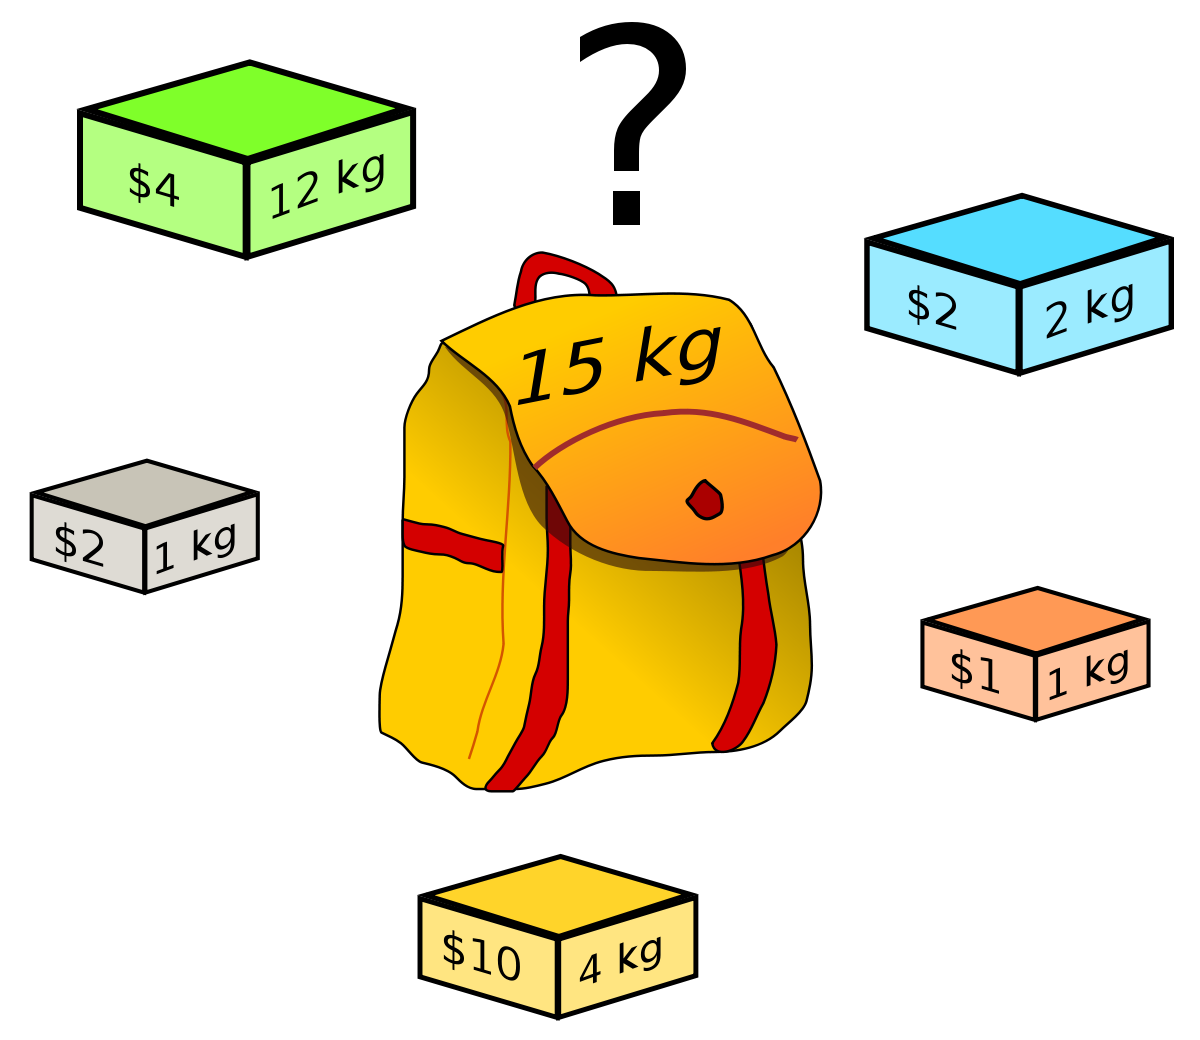
\includegraphics[scale=0.1]{Knapsack}

\end{document}

